% arara: pdflatex: {synctex: yes}
% arara: makeindex: { style: SpecificImpulseEff }
% arara: biber
% arara: pdflatex: {synctex: yes}
% arara: pdflatex: {synctex: yes}
% arara: clean: {files: [SpecificImpulseEff.aux, SpecificImpulseEff.idx, SpecificImpulseEff.ilg, SpecificImpulseEff.ind, SpecificImpulseEff.log, SpecificImpulseEff.bbl, SpecificImpulseEff.bcf, SpecificImpulseEff.ist, SpecificImpulseEff.blg, SpecificImpulseEff.run.xml]}
%
\documentclass[twocolumn]{memoir} %twocolumn
\usepackage[utf8]{inputenc}
\usepackage[english]{babel}
\usepackage[T1]{fontenc}
% Nicer default font (+ math font) than Computer Modern for most use cases
\usepackage{mathpazo}
\usepackage{graphicx}
\usepackage{caption}
\usepackage{xcolor} % Allow colors to be defined
\usepackage{enumerate} % Needed for markdown enumerations to work
\usepackage[]{geometry} % Used to adjust the document margins
\usepackage{amsmath} % Equations
\usepackage{amssymb} % Equations
\usepackage{booktabs}  
\usepackage{longtable}
\usepackage{wrapfig}
\usepackage{dblfloatfix}
\usepackage{hyperref}
\usepackage{cleveref}
\usepackage{tikz} 
\usepackage{pgf}
\usepackage{float}

\providecommand{\tightlist}{%
  \setlength{\itemsep}{0pt}\setlength{\parskip}{0pt}
}

\renewcommand*\familydefault{\sfdefault}

\chapterstyle{demo2}
\setlrmarginsandblock{0.75in}{0.75in}{*}
\setulmarginsandblock{1in}{*}{1}
\checkandfixthelayout 

\graphicspath{ {./imgs/} }


\title{Rocket parameters and Efficiency}
\author{Jonny Dyer}
 
\begin{document}

\chapter*{Rocket parameters and Efficiency}

\subsubsection{Assumptions for topics already
covered}\label{assumptions-for-topics-already-covered}

\begin{itemize}
\item
  Equation for thrust -

  \begin{itemize}
  \item
    $T = \dot{m}_{in}(U_e - U_0) + (P_e - P_0)A_e + \dot{m}_pU_e$
  \item
    Reduces to $T = (P_e - P_0)A_e + \dot{m}_pU_e$ for rocket case
  \end{itemize}
\item
  Rocket equation - $\Delta V = C \ln \frac{m_0}{m_i}$
\item
  Isentropic flow through nozzles, critical flow, supersonic flow in de
  laval nozzle
\end{itemize}

\section{Effective Exhaust Velocity and Specific Impulse}\label{c-and-isp}

Now that we have covered the basic mechanics of thrust and the
isentropic nozzle relations we will begin to show how these apply to
rockets by defining a set of convenient parameters.

\begin{figure}[H]
    \centering
    \includegraphics*[width=0.95\columnwidth]{imgs/nozzle_pressure}
    %\input{imgs/cstar_gamma.pgf}
\end{figure}

Let's start by remembering that, for a rocket

\begin{equation}T = (P_e - P_0)A_e + \dot{m}_pU_e
\end{equation}
%
Our intuition tells us that a good parameter for the effectiveness of a
rocket is the quotient of thrust (what we want) with propellant mass
flowrate (what we have to pay):

\begin{equation}\frac{T}{\dot{m}} = (P_e - P_0)\frac{Ae}{\dot{m}} + U_e
\end{equation}
%
This parameter is called effective exhaust velocity,

\begin{equation}
    C = \frac{T}{\dot{m}}
\end{equation}
%
and is one of the most important relations in rocketry.
It figures prominently in the Rocket Equation

\begin{equation}\Delta V = C \ln \frac{M_0}{M_f}
\end{equation}
%
which we will be derived in a couple lectures.

If we assume $T$ and $\dot{m}$ are completely independent (which we
will see is not always true), we can also interpret $C$ as

\begin{equation}C = \frac{\int T dt}{\int \dot{m} dt} = \frac{I}{M_p}
\end{equation}
%
which is how much total impulse we get from a unit mass of propellant.
This interpretation points to a very closely related parameter called
Specific Impulse, $I_{sp}$:

\begin{equation}I_{sp} = \frac{C}{g_0} = \frac{T}{g_0\dot{m}}
\end{equation}

Notice that $I_{sp}$ is just $C$ normalized by Earth's gravitational
acceleration with overall units of seconds. While the unit is at first a bit
non-sensical, $I_{sp}$ makes sense when you consider your propellant
consumption as a weight flowrate rather than a mass-flowrate and so you
are dividing thrust (a force) by weight flowrate (force per time) to
arrive at a time. The etymology of $I_{sp}$ is rooted in the fact that
for imperial units we typically work in lbm. rather than slugs.

And while weird at first, the units of seconds do have some intuitive
utility. For a rocket with $I_{sp} = 100 \text{s}$ a unit mass, $m$
of propellant can generate enough thrust to support its weight in Earth's
gravity for 100 seconds or 100 times its weight for one second.

%\begin{wraptable}{l}{0.9\linewidth}
\begin{table*}[h]
    \centering
    \begin{tabular}{lll}
    \toprule
    Technology                    & Isp (s)        & Exhaust Velocity (m/s)  \\
    \midrule
    Electric Propulsion           & 1000 - 10,000  & 9,800 - 98,000  \\
    Nuclear Thermal / Beamed Energy Propulsion & 600 - 1,000  & 5,900 - 9,800  \\
    Bipropellant Chemical Propulsion           & 200 - 500    & 2,000 - 4,900  \\
    Monopropellant Chemical Propulsion         & 100 - 250    & 980 - 2,450  \\
    Cold Gas Propulsion                        & 10 - 120     & 100 - 1,150  \\
    \bottomrule
    \end{tabular}
\caption{Table 1 - Representative effective exhaust velocities for different propulsion technologies}
\label{t:tech_c}
\end{table*}

Specific impulse is popularly spoken of as the "gas mileage" for a
rocket cycle and this is fairly reasonable - it fundamentally indicates
how much bang for the buck you get. I'll jump the gun just a bit for the
sake of intuition and give some typical $I_{sp}$ values for different
types of propulsion in ~\cref{t:tech_c}.

This is all well and good, but all we have really done at this point is
some algebra. What we really are interested in as engineers is how do I
get the most gas mileage out of my rocket. And for that discussion,
we'll first define another couple useful parameters.

\section{$c*$}\label{c}

We will go back, for a moment, to choked compressible flow. With the
isentropic flow equations and the $M=1$ choked condition, we can
derive (assuming constant $C_p$, $C_v$ and $R$):

\begin{equation}\dot{m} = \rho_c a^* A^*  = \rho_t \left[ \frac{\rho_c}{\rho_t}\right]a_0 \left[ \frac{a^*}{a_t}\right]A^* = \frac{P_t A^*}{\sqrt{\frac{R T_t}{\gamma}}} \left[\frac{\gamma + 1}{2}\right]^{\frac{2(\gamma-1)}{\gamma+1}}
\end{equation}
%
remembering that the $t$ subscript denotes the total or stagnation
condition and the $c$ subscript denotes choked ($M=1$) condition.
This is a very useful relationship as it allows us to compute the mass
flowrate through a choked nozzle as a function of only nozzle throat
area, $A^*$, ideal gas properties and the stangation condition
temperature and pressure.

Let's define a new parameter, called characteristic velocity and denoted
$c^{*}$ using this result:

\begin{equation}c^* = \frac{P_t A^*}{\dot{m}} = \sqrt{\frac{R T_t}{\gamma}}\left[\frac{\gamma + 1}{2}\right]^{\frac{\gamma + 1}{2(\gamma - 1)}}
    \label{eq:cstar}
\end{equation}

\begin{figure}[H]
    \includegraphics[width=0.9\columnwidth]{cstar_diagram}
    \caption{$c^*$ parameters of interest.  $\dot{m}$, $P_t$ and $A^*$ are all easily 
    measureable.  $T_t$ is difficult due to the extremely high temperatures of chemical
    rockets.}
\end{figure}

$c^*$ is useful far beyond simple choked flow considerations because
it can be both \textbf{measured} and \textbf{computed}. And indeed the
equation above shows this directly - the LHS is a function 
measure-able variables stagnation pressure $P_t$\footnote{In a finite sized rocket chamber we are not actually measuring stagnation pressure because there will be non-zero gas velocity.  For reasonable \emph{contraction ratios}, $A_1/A^*$, this is a small effect and it can be mostly corrected analytically using isentropic flow relations}, area $A^*$ and mass flowrate $\dot{m}$. The RHS is a
function of intrinsic gas properties $\gamma$, $R$ and stagnation
temperature. $c^*$ gives us the tools to calculate a parameter (RHS)
that we can go and easily measure in the lab (LHS).

Given that $c^*$ depends on $\gamma$, $R$ and $T_t$ it is essentially a function only of the working fluids thermodynamic properties and stagnation (chamber) state.  This is not 100\% true - when we get to combustion we will see how a (weak) dependency on pressure comes back into $c^*$, but for conceptual purposes we should think of $c^*$ this way - as only a function of intrinsic thermodynamic properties of our propellants.

And so finally we come to a very interesting result regarding the
functional dependence of $c^*$:

\begin{equation}c^* = f(T_t, R, \gamma)
\end{equation}
%
$R$ is the specific gas constant $R = \frac{R_u}{M_w}$ which is
inversely dependent on gas molecular weight, $M_w$. Thus

\begin{equation}c^* \propto \sqrt{\frac{T_t}{M_w}}
\end{equation}
%
Moreover $T_t$ is related to the gas internal stagnation enthalpy by
$\Delta h_t = \int_{T_0}^{T_t} C_p dT$ and so we should see $T_t$ as
a representation of the \textbf{energy content} of the rocket gasses.

The effect of $\gamma$ on $c^*$ is a bit more subtle. $\gamma$ is
fundamentally related to the number of vibratory degrees of freedom a
molecule has. For monatomic systems (such as helium or atomic hydrogen)
$\gamma$ assymptotes to an upper limit of 1.66. For most simple
diatoms (nitrogen, oxygen, hydrogen) it is around 1.4 and for larger
molecules or those with more complex bonding it is lower. For the
conditions we are interested in within a rocket, we wouldn't expect to
find $\gamma$ much lower than 1.1.

\begin{figure}[H]
    \includegraphics[width=0.48\textwidth]{imgs/cstar_gamma.pdf}
    %\input{imgs/cstar_gamma.pgf}
    \caption{$c^*$ shows only a weak dependence on $\gamma$}
\end{figure}

The plot below shows the effect of $\gamma$ on $c^*$ which is fairly
limited compared with $T_t$ and $M_w$. And so if you take one thing
away from this discussion, remember that

\begin{equation}c^* \propto \sqrt{\frac{\Delta h_t}{\overline{C_p} M_w}}
\end{equation}

\section{$C_f$}

Ok, that's interesting, but for the purposes of rocket performance we
want \(C\) not \(c^*\). Take a look at the definition of \(c^*\) and it
looks a lot like our definition of effective velocity and specific
impulse above:

\begin{equation}c^* = \frac{P_t A^*}{\dot{m}} \sim \frac{T}{\dot{m}} = C
\end{equation}
%
and indeed \(c^*\) and \(C\) \textbf{are} closely related.

In order to see how, let's define another new parameter, \(C_f\) that
related thrust to the nozzle throat area and rocket total pressure:

\begin{equation}C_f = \frac{T}{P_t A^*}
\end{equation}
%
In prose this says:
%
\begin{quote}
    \emph{\(C_f\) represents the amount of thrust a rocket can produce given the
stagnation pressure of its propellants and a useful characteristic fluid
    area - the choked area of its nozzle.}
\end{quote}

Stated differently it is a measure of how effectively we take the
stagnation pressure we generate in the chamber and turn it into thrust.

And since \(c^*\) is also defined by chamber pressure and nozzle throat
area, \(C_f\) becomes the connection between \(C\) and \(c^*\):

\begin{equation}
    C = \frac{T}{\dot{m}} = \frac{C_f P_t A^*}{\dot{m}} = C_f c^*
    \label{eq:C}
\end{equation}

But why split \(C\) into \(C_f\) and \(c^*\) this way?

Remember that \(c^*\) represents the potential of the rocket propellants
themselves to create thrust and essentially depends exclusively on the
thermodynamic characteristics of those propellants. \(C_f\) represents
how well our nozzle can convert the propellant's latent utility into
real thrust and thus depends almost exclusively on the physical nature
of our nozzle. And so as we go about maximizing \(C\), we can divide
that into two separate problems - one of picking propellants (\(c^*\))
and the other of chosing system pressures and nozzle geometry (\(C_f\)).

Since the primary role of the nozzle is to convert gasses into thrust
\(C_f\) can also be seen as a measure of the "goodness" of the nozzle.
It is called \textbf{thrust coefficient}.

\(C_f\) can be expanded from its definition above:

\begin{equation}
    \begin{split}
        C_f = \frac{C}{c^*} &= \frac{(P_e - P_0)\frac{A_e}{\dot{m}} + U_e}{\frac{P_t A^*}{\dot{m}}} = \frac{P_e - P_0}{P_t}\frac{A_e}{A^*} + \frac{U_e}{c^*} \\
        & \Rightarrow \left(1 - \frac{P_0}{P_e}\right)\frac{P_e A_e}{P_t A^*} + \frac{U_e}{c^*}
    \end{split}
\end{equation}

It is worth noting that, like the thrust equation, there are two pieces
to \(C_f\): $\left(1 - \frac{P_0}{P_e}\right)\frac{P_e A_e}{P_t A^*}$ is representative
of thrust created through pressure force and \(\frac{U_e}{c^*}\) is
representative of the contribution of gas momentum to thrust. We will
refer to these two components when we discuss optimal nozzle expansion
in a minute.

Beyond this things get a little messy and different people attack the
derivation different ways. Rather than putting a whole bunch of alegbra
in here, I'm going to provide you the tools needed to compute \(C_f\)
practically.

\(\frac{U_e}{c^*}\), \(\frac{P_e}{P_t}\) and \(\frac{A_e}{A^*}\) are all
related to the isentropic expansion of gasses through the nozzle to its
exit. The exit mach number, \(M_e\) thus becomes the common parameter
and using classic isentropic relations we can derive the functional
relationship of each with \(M_e\) as the independent variable:

\begin{equation}
    \frac{U_e}{c^*} = \frac{\gamma M_e}{\sqrt{1 + \frac{\gamma - 1}{2}M_e^2}}\left[\frac{\gamma + 1}{2}\right]^{\frac{\gamma + 1}{-2(\gamma-1)}}
\end{equation}

\begin{equation}
    \frac{P_e}{P_t} = \left(1 + \frac{\gamma - 1}{2}M_e^2\right)^{\frac{-\gamma}{\gamma-1}}
\end{equation}

\begin{equation}
    \frac{A_e}{A^*} = \left[\frac{\gamma + 1}{2}\right]^{\frac{\gamma + 1}{-2(\gamma - 1)}} \frac{\left(1 + \frac{\gamma-1}{2}M_e^2 \right)^{\frac{\gamma + 1}{2(\gamma - 1)}}}{M_e}
\end{equation}

This is a useful form because it shows very clearly that
\(\frac{U_e}{c^*}\), \(\frac{P_e}{P_t}\) and \(\frac{A_e}{A^*}\) are not
all independent (they all depend on \(M_e\)). In fact the dimensionality
of this set is one - picking a number for any one of these directlys
sets the others. Furthermore note that these equations, unlike \(c^*\),
have \textbf{no dependency on stagnation temperature or molecular weight and
thus no direct dependency on propellant properties}. They do depend on
\(\gamma\) which is a property of the working fluid but as with \(c^*\),
the dependence is not terribly strong and is really set for us by the
propellant choice we made in optimizing \(c^*\).

I'd like to look at how the parameter we can control directly,
\(A_e/A^*\), affects the others and \(C_f\). Using the equations
above, we will sweep through \(M_e\) and compute the other parameters
directly.

\begin{figure}[H]
    \includegraphics[width=0.48\textwidth]{imgs/Cf_5_7.pdf}
    %\input{imgs/cstar_gamma.pgf}
    \caption{Relationship of the components of $C_f$ to each other and to $C_f$ itself.}
\end{figure}

Note that the momentum component grows as exit pressure decreases because the gasses are accelerated further before release.  Conversely, the pressure component decreases as exit pressure decreases for obvious reasons.  In fact the pressure component of $C_f$ takes on negative values for exit pressures below ambient - this is called over-expansion.

$A_e/A^*$ increases monotonically with decreasing exit pressure - this simply represents the fact that to achieve lower exit pressures we must use a larger nozzle expansion ratio.

Finally note that \(C_f\) reaches a maximum where \(P_e/P_0 = 1\). This
is called optimal expansion. It is a fundamental result in rocket theory
and can be stated:

\begin{quote}
    \emph{Rocket effective exhaust velocity (and therefore specific impulse) is
maximized when the nozzle expands the exhaust gasses such that they
    match the local pressure at the nozzle exit.}
\end{quote}

In general, we want to design a rocket nozzle to match
the exit pressure to ambient pressure. This is difficult to do for a
rocket ascending through the atmosphere where the pressure is
continuosly changing. For traditional nozzles, a compromise that looks
at the average performance over the ascent pressure profile is often
chosen.

\begin{figure}[H]
    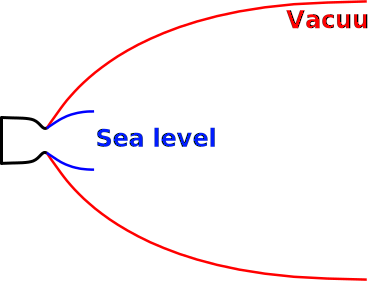
\includegraphics[width=0.9\columnwidth]{nozzle_sl_vacuum.pdf}
    \caption{Note the size difference between a sea-level and vacuum- optimized 
    nozzle.  The rocket itself is identical except for the nozzle expansion.}
\end{figure}

And since the way we lower exit pressure is with a bigger expansion
ratio, \(\epsilon = \frac{A_e}{A^*}\), this result explains why upper
stage "vacuum nozzles" are so much bigger than first stage "sea-level"
nozzles as can be seen in graphic above and the side-by-side of the
SpaceX Merlin 1D vacuum (left) and Merlin 1D sea-level (right) engines:

\begin{figure}[H]
    \includegraphics[width=0.9\columnwidth]{merlin}
    \caption{SpaceX' Merlin engine has very different size nozzles for its first
    and second stage even though the engine itself is nearly identical.}
\end{figure}

So what actually happens when a nozzle is under- or over- expanded?  In a subsconic
(incompressivle) jet, the fluid dynamics allow for communication of information upstream
and the pressure distribution in the nozzle would relax to a state where $P_e = P_0$. 
In supersonic (compressible flow), pressure information travels more slowly than the fluid
velocity so there is no information transfer upstream.  In order to equilibrate pressure with
the ambient, a set of expansion or compression waves form from the exit of the nozzle.  

\begin{figure}[h]
    \includegraphics[width=0.9\columnwidth]{overExpanded.pdf}
    \caption{In a super-sonic exhaust stream, expansion or compression waves form to
    equilibrate the jet pressure to the surrounding pressures.}
\end{figure}

Due to flow radial inhomogeneity in the flow in real nozzles, there will always be some
equilibration wave structure at the exit.  The pattern of compression and expansion waves
and associated changes in gas temperature and luminosity are what are generate \emph{Mach
Diamonds} in the exhaust stream.

\begin{figure}[h]
    \includegraphics[width=0.9\columnwidth]{mach_diamonds}
    \caption{An example of mach diamonds in the plume of one of Stanford's research
    hybrid rockets}
\end{figure}


\section{$c^*$ Efficiency}
Due to imperfect mixing, combustion, chamber heat-loss and other effects the
realized rocket performance is typically less than that computed theoretically.
This will be reflected in the rocket thrust, effective velocity and $c^*$ and potentially
$C_f$.

Becuase many of the larger losses are associated with the process of combustion
in the chamber, the non-ideal performance is most easily and directly measured in
$c^*$.  It is with this in mind that \emph{$c^*$ efficiency} is defined:

\begin{equation}
    \eta_{c^*} = \frac{c^*_{measured}}{c^*_{ideal}} = \frac{P_t A^*}{\dot{m}_p c^*_{ideal}}
\end{equation}
%
where $c^*_{ideal}$ is computed using \cref{eq:cstar} for simple substances or, more
commonly, using a complex chemical equillibrium code as will be discussed in the next
lecture.

Optimizing $\eta_{c^*}$ becomes a primary activity in the development of a rocket
engine, often consuming a singificant fraction of the development budget and time.  In
liquid rockets this might manifest as injector tuning, while in a solid rocket it is
attacked by adjusting propellant composition, ratios and particle sizes.

\section{Putting it all together}\label{putting-it-all-together}

The separation of \(C\) into \(c^*\) and \(C_f\) separates
concerns between propellant thermodyanmics in \(c^*\) and nozzle
physical parameters in \(C_f\).

Let's quickly compute \(C\), \(c^*\) and \(C_f\) to get a sense of
how we would begin to use them practically. Assume we start with a
plenum full of room-temperature, high pressure gas and then vent it
into vacuum through a nozzle. 

Now let's compute \(c^*\), \(C_f\) and then \(C\). For now we will
assume optimal expansion ($P_0/P_e = 1$) and calculate the associated area ratio. A
useful relation we will use to determine \(M_e\) is:

\begin{equation}
    M_e^2 = 2\left(\frac{\frac{Pe}{Pt}^{\frac{1-\gamma}{\gamma}}-1}{\gamma-1}\right) = 2\left(\frac{\left(\frac{P_e}{P_0}\frac{P_0}{P_t}\right)^{\frac{1-\gamma}{\gamma}}-1}{\gamma-1}\right)
\end{equation}

\begin{table}[h]
\centering
\begin{tabular}{llllll}
\toprule
Name & $\gamma$ & $M_w$ & $c^*$ (m/s) & $C_f$ & $C$ (m/s) \\
\midrule
$N_2$ & 1.40 & 28 & 434.4 & 1.26 & 546.4 \\
$H_2$ & 1.41 & 2 & 1621.5 & 1.26 & 2039.2 \\
He & 1.66 & 4 & 1085.2 & 1.25 & 1356.2 \\

\bottomrule
\end{tabular}
        
\caption{$c^*$, $C_f$, $C$ for several pure gasses at room temperature,
        $P_0/P_e = 1$ and $P_0/P_t = 0.1$. Note how $C_f$ is essentially
        constant despite the differences in gas properties while $c^*$ and
        $C$ vary substantially.}    

\end{table}

This simple exercise confirms what we said before - $c^*$ depends on the nature of working fluid while $C_f$ is largely fixed by the nozzle parameters.  Another interesting conclusion from this is that even before we get to chemistry, we can
see how wonderful of a working fluid Hydrogen is due to it's low
molecular weight. Remember this because hydrogen will emerge again and
again as we talk about rockets.

If we expand \cref{eq:C} and simplify we arrive at a useful form for $C$:

\begin{equation}
    C = \sqrt{\frac{2 \gamma}{\gamma-1}\frac{R_u T_t}{M_w}\left[1 - \left(\frac{P_e}{P_t}\right)^{(\gamma - 1)/\gamma}\right]}
    \label{eq:C_exp}
\end{equation}
%
In \cref{eq:C_exp} we can see all the impacts of propellant choice and 
nozzles on effective exhaust velocity.  The term involving $T_t$ and $M_w$ clearly
shows the effect of propellant choice on $C$, as we noted with $c^*$ earlier.
The term involving $\frac{P_e}{P_t}$ demonstrates the impact of the system pressures
and nozzle geometry we choose.  \cref{fig:C} summarizes all of this.

\begin{figure}[h]
    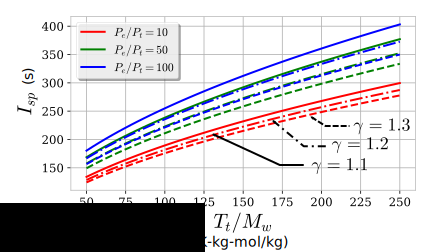
\includegraphics[width=\columnwidth]{C_exp}
    \caption{How specific impulse varies}
    \label{fig:C}
\end{figure}

\section{Energy and efficiency}\label{energy-thermodynamics-and-efficiency}

So far we have concentrated on propulsion primarily from a conservation
of momentum perspective. But there are a lot interesting observations to
be made when we look at the thermodynamics of propulsion as well.

With rocket propulsion and things in space we are talking about
\textbf{a lot of energy} and to put that in to context, let's see how
much energy our Low Earth Orbit satellite ends up with.

An object moving in a conservative potential field (like Earth's
gravity) has total energy:

\[E = \text{KE} + \text{PE} = \frac{m v^2}{2} + \frac{GMm}{r}\]

or in \textbf{mass-specific energy}

\[\epsilon = \frac{v^2}{2} + \frac{GM}{r}\]

In the case of our satellite in a circular Low Earth Orbit this comes
out to:

\[\epsilon = \frac{v^2}{2} + \frac{\mu}{r_0} - \frac{\mu}{r} = 29.1 \text{MJ/kg} + 4.5 \text{MJ/kg} = \mathbf{33.6} \textbf{MJ/kg}\]

Again note how much of this is due to the orbital velocity of the
rocket. And to put in context just how much energy this is, it is
equivalent to:

\begin{itemize}
\item
  1000x the specific energy of a Jet airliner at 650MPH
\item
  5x the specific chemical energy content of nitroglycerin
\item
  3x the required specific energy to melt aluminum
\end{itemize}

It is no wonder that not much is left when object with this much energy
slams into the atmosphere!

\section{Rocket efficiency}\label{rocket-efficiency}

Clearly there is a lot of energy being liberated in rocket engines in
order to put things into space. But how efficient are they?

There are different ways to define energy efficiency, but the the first
we'll look at is the \textbf{thermal efficiency} or how effectively a
rocket takes input energy and converts it to gas kinetic energy:

\[\eta_{thermal} = \frac{\dot{W}_{exhaust}}{P_{in}} = \frac{\dot{m}C^2}{2P_{in}}\]
where \(P_{in}\) is the amount of energy being liberated in time to
power the rocket whether it be latent, chemical, nuclear or electrical energy. In
the case of chemical rockets we can define it as the energy released by
the propellants when they combust or:

\[P_{in} = \dot{m} \Delta h\]
%
where $\Delta h$ is the amount of thermal energy going into the rocket chamber.

Substituting \cref{eq:C_exp} gives

\begin{equation}
    \eta_{thermal} = \frac{\frac{2 \gamma}{\gamma-1}R T_t\left[1 - \left(\frac{P_e}{P_t}\right)^{(\gamma - 1)/\gamma}\right]}{2 \Delta h}
    \label{eq:eta_therm}
\end{equation}
%
Because
%
$$T_t \sim \frac{\Delta h}{\overline{C_p}}$$
%
we can subsitute such that

\begin{equation}
    \eta_{thermal} = \frac{\gamma}{\gamma-1}\frac{R}{\overline{C_p}}\left[1 - \left(\frac{P_e}{P_t}\right)^{(\gamma - 1)/\gamma}\right]
\end{equation}
%
And finally recognizing that for an ideal gas

$$\frac{R}{\overline{C_p}} = \frac{\gamma - 1}{\gamma}$$
%
and for a perfectly isentropic nozzle expansion process
%
$$\frac{T_e}{T_t} = \frac{P_e}{P_t}^{(\gamma - 1)/\gamma}$$
%
we see that \cref{eq:eta_therm} reduces to the Carnot efficiency.

\cref{fig:eta_therm} shows $\eta_{thermal}$ as a function of $P_t/P_e$:

\begin{figure}[h]
    \includegraphics[width=\columnwidth]{eta_therm}
    \caption{How specific impulse varies}
    \label{fig:eta_therm}
\end{figure}

This is pretty good for a heat engine and a lot of early rocket work focused on optimizing thermal efficiency.  And thermal efficiency will matter when we get to electric propulsion, but it is less useful a construct for chemical rockets where it is largely defined by the propellant properties rather than the machine they burn in.  Furthermore the efficiency of
accelerating gasses is not really what we care about - we care about the
efficiency of accelerating the vehicle.

To understand that, we will define another, more useful effiency metric, called
\textbf{propulsive efficiency} as such

\[\eta_{prop} = \frac{\dot{W}_{r}}{\dot{W}_{r} + \dot{W}_{exhaust}} = \frac{Tv}{Tv + \frac{1}{2}\dot{m}(C - v)^2}\]
%
or the fraction of total work that actually goes to accelerating the
vehicle.

\[\frac{Tv}{Tv + \frac{1}{2}\dot{m}(C - v)^2} = \frac{\dot{m}C v}{\dot{m}\left[C v + (C-v)^2\right]}\]

\[\rightarrow \eta_{prop} = 2\frac{\frac{v}{C}}{1+(\frac{v}{C})^2}\]
%
The overall efficiency is \[\eta = \eta_{thermal}\eta_{prop}\]

A small example demonstrating how \(\eta\) varies over ratio of vehicle
speed to exhaust speed, \(\frac{v}{C}\) is shown below.

\begin{figure}[H]
    \includegraphics[width=0.9\columnwidth]{prop_eff}
\end{figure}

And here we see another interesting result much like optimal nozzle
expansion. The rocket is most efficient when the exhaust velocity equals
the vehicle velocity. This is actually quite intuitive - in this
condition the exhaust gasses are left with zero velocity in the static
frame. There is no residual kinetic energy in the exhaust so all of it's
kinetic energy have been transferred to the vehicle. Anywhere else the
exhaust is left with residual kinetic energy which is a loss.

Propulsive efficiency will come back in a big way when discuss electrical propulsion as it is very important to system optimization.

\section{Energy losses}\label{energy-losses}

Finally let's also look at where the inefficiencies are for a typical launch vehicle powered by a chemical engine with \(I_{sp} = 340\) s and moving at 5,000 m/s for intuition.

\begin{figure}[H]
    \includegraphics[width=\columnwidth]{sankey}
\end{figure}
%
Notice that almost half of the chemical energy is unavailable for conversion to work due to second law of thermodynamics.  This is expected given the Carnot efficiency we developed earlier.  The biggest contributor after second law loss is residual exhaust kinetic energy which we saw is something is minimized when $V/C = 1$.  The other losses are quite small and we can say

\begin{quote}
    \emph{When a rocket operates with exhaust velocity near vehicle velocity,
    it is a surprisingly efficient heat engine}
\end{quote}

\end{document}
